%!TEX root = ../thesis.tex
%*******************************************************************************
%****************************** Third Chapter **********************************
%*******************************************************************************
\chapter[In-situ study of avalanches]{Audiovisual experience in dislocation avalanches: a coupled in situ study of strain bursts and acoustic emission \hyperref[paper:A1]{[O4]}} \label{chapter:in_situ}

% **************************** Define Graphics Path **************************
\ifpdf
    \graphicspath{{Chapter3/Figs/Raster/}{Chapter3/Figs/PDF/}{Chapter3/Figs/}}
\else
    \graphicspath{{Chapter3/Figs/Vector/}{Chapter3/Figs/}}
\fi

Micron-scale plastic deformation of crystalline materials is characterised by stochastic strain burst \cite{PhysRevLett.89.165501,weiss2003three,PhysRevLett.93.195507,1742-5468-2005-08-P08004,Zapperi2012}, a phenomenon does not happen in bulk samples. Stress-strain curves vary from sample to sample so in order to obtain a detailed picture of the stochastic, intermittent deformation behaviour, numbersome specimens in the micron-scale are required for testing. The scientific to mass fabricate such specimens is already realised but it is still a huge technological challenge to achieve it in an effective way. To this end in this study an improved FIB fabrication method is proposed to prepare non-tapered micropillars more efficiently than with other methods. An in situ nanoindentation device is also developed allowing high-accuracy force and displacement measurements with high sampling rates and high accuracy sample positioning. The avalanche-like motion of the single crystalline emerges from the collective motion of the dislocations and can be observed as step-like stress decreasements on the stress-strain curves. As a novel application an acoustic emission (AE) \nomenclature[z-AE]{AE}{acoustic emission} detector was also mounted onto the setup to study the plastic response of micropillars. This technique firmly supports the SEM's in situ information acquisition as it is particularly sensitive to the collection motion of dislocations observed as the stress-steps on the stress-strain curves.

\section{Motivation}
The miniaturisation of electromechanical devices has reached a level in 21st century where further research are desired to investigate the plastic properties of micron-sized specimens \cite{doi:10.1080/14786430600567739,NG20081712,doi:10.1080/14786430802132522,doi:10.1146/annurev-matsci-082908-145409,ZHOU20117673}. These micron-sized components are used in micromachined inertial sensors \cite{704269} and also in cantilever transducers as a platform for chemical and biological sensors \cite{doi:10.1063/1.1763252}. The demand for ever smaller elements requires the detailed understanding of the underlying physical processes during plastic deformation on a similar size-scale.

Plastic deformation is realised by single dislocations only in the most spare cases. In (large enough) single crystals the typical process is realized by the collective motion and rearrangement of dislocations. The stress-strain curve for bulk materials is smooth and characterised by the mechanical and chemical properties of the specimen investigated. These curves are reproducible because the stochastic noise from dislocation ensembles is marginal, the size of the dislocation ensemble taking part at a time in plastic deformation in is negligible compared to total number of dislocation -- at least under the commonly used resolutions. This allows predicting the material behaviour with high accuracy. In contrast, at micrometer scales the stochastic noise from dislocation ensembles are not marginal but plays a major role in the plastic response, when the size of dislocation microstructure is in the same order of magnitude as the sample size. The activation of dislocation ensembles can be characterised by stochastic processes leading to a discontinuous plastic response. This behaviour makes it impossible to predict the exact stress-strain curve on an elementary level -- only statistical statements can be formed, therefore a statistical approach must be applied when it comes to specimen testing at this size scale.

The first remarkable evidences of intermittent crystal plasticity phenomena were observed in ice single crystals under creep deformation \cite{miguel2001intermittent,weiss2000statistical}, however, these experiments gave only an indirect possibility of investigations as they only used AE detection for the observation of the strong signals. A couple of years later SEM experiments (Ni single-crystalline micropillar compression \cite{Uchic986,Dimiduk1188,doi:10.1146/annurev-matsci-082908-145422}) were conducted to find out that the plastic response of single crystal micropillars are dominated by instabilities in the form of strain jumps. The fact that micron sized samples behave differently than bulk materials raises the following questions \cite{ARZT19985611,GREER2011654,ISPANOVITY20136234}.
\begin{enumerate}
\item Is there a limit between microscopic and macroscopic deformation?
\item What are the good definitions for material strengths parameters, e.g.\ yield point or ultimate tensile strength?
\end{enumerate}

The statistical nature of this behaviour requires large number of samples to be tested. FIB milling \cite{0960-1317-11-4-301} is one of the most frequent method for fabricating micropillars, i.e.\ micron-sized pillars. During the fabrication process the sample is under visual control of a SEM providing a conventional way for milling, and is not limited to material or crystal type, however, slight differences in the technique may be required. FIB was introduced as a comprehensive method to fabric wide range of shapes and materials under different circumstances individually, as per request, meaning that FIB is a time consuming "Jolly Joker" technique. FIB-less techniques have been also introduced \cite{doi:10.1021/nl902872w,PhysRevLett.104.135503} to shorten fabrication time of micropillars, but they lack the possibility to control the properties of dislocation-structure in the micropillars. Moreover it cannot used on arbitrary material and pillars are only semi-fixed to the surface due to the underlying technique, which leaves FIB-less technique an unpracticed method in micropillar fabrication for the purpose of investigation micron-scale plasticity.

There are two main approaches commonly used in FIB milling to fabricate micropillars \cite{HUTSCH201449}. They are summarised in Table~\ref{tab:fib}.

\begin{table}[htp]
\centering
\caption[FIB approaches]{The two major FIB approaches used before 2015 are compared. The method used in this study combines the two.}
\label{tab:fib}
\begin{tabular}{lll}
\hline
\multicolumn{1}{c}{Approach} & \multicolumn{1}{c}{lathe}                                                                                                                                                                                                           & \multicolumn{1}{c}{annular}                                                                                                                     \\ \hline
Directions                   & \begin{tabular}[c]{@{}l@{}}the ion beam is\\ almost perpendicular\\ to the axis of the micropillar;\\ the sample is rotated\\ around the axis of the pillar\\ forming a pair of skew lines\\ with the axis of ion beam\end{tabular} & \begin{tabular}[c]{@{}l@{}}the pillar axis is always parallel\\ to the ion beam axis;\\ the sample is rotated\\ around the pillar axis\end{tabular} \\ \hline
Shape                        & \begin{tabular}[c]{@{}l@{}}strong control on shape;\\ cylindrical shape\\ can be obtained if\\ the stage is rotating\\ at a constant speed\\ while the beam is on\end{tabular}                                                      & \begin{tabular}[c]{@{}l@{}}weak control on shape;\\ more or less tampered shape;\\ cylindrical shape is preferred\end{tabular}                  \\ \hline
Advantages                   & perfect shape control                                                                                                                                                                                                               & \begin{tabular}[c]{@{}l@{}}time effective;\\ smaller ion damage and pollution\end{tabular}                                                      \\ \hline
\end{tabular}
\end{table}

The new method described here combines the two techniques so that it is considerably faster and yet still suitable for a wide range of pillar shapes \cite{wurster2015novel}.

The new fabrication method was needed to produce micropillars with moderate resources in order to produce such an amount of them which is suitable for statistical analysis \cite{ispanovity2010submicron}.

In our demonstrative work compression tests were performed on micropillars fabricated on the surface of a bulk material of Al - 5\% Mg alloy which exhibits the Portevin-Le Chatelier (PLC) \nomenclature[z-PLC]{PLC}{Portevin-Le Chatelier} effect \cite{TABATA1980795,chinh2000critical,GUBICZA200455,1468-6996-12-6-063001}. In this type of alloy the stress-strain curve of even for bulk samples show intermittent plastic response to external shear which originates from the periodic pile-ups and break-outs (pinning and depinning) of dislocations pinned at the solute atoms acting as obstacles for mobile dislocations \cite{GUBICZA200455,1468-6996-12-6-063001}. Compared to non-PLC dislocation avalanches, which cannot envisaged as a depinning phenomenon \cite{PhysRevLett.112.235501}, PLC dislocation avalanches generate stronger AE signals, which helps to catch AE signals and couple them with the stress-drops measured on the stress-strain curves.

\section{Sample preparation}
In this study we focus on investigating collective dislocation phenomena, therefore two properties of the sample are desired. At one hand large dislocation density serves our goal in the term of stronger AE signals, and on the other hand small enough samples are preferred which provides isolable stress-drops in the stress-strain curves. Dislocation density in FCC metals, such as Al, varies from \SIrange{e11}{e14}{/m^2}, therefore the mean dislocation spacing varies from \SIrange{0.1}{3}{\micro\meter}. Dislocation patters, i.e.\ the cell-like structure is often formed in these materials with a characteristic size scale of 10 times the mean dislocation spacing, therefore a specimen size not larger than \SIrange{1}{30}{\micro\meter} is desired. It is worth to mention that although dislocation density and the characteristic size of the cell-structure depend on the applied plastic strain and sample size, their ratio remains the same \cite{doi:10.1080/14786435.2014.906755,el2015unravelling}.

In situ micropillar deformation demands high requirements on the sample. Outstanding technological proficiency is required to prepare such samples which meet all those requirements. Without going into details the following procedure was performed to achieve the appropriate surface quality, specimen size, initial dislocation density and orientation.
\begin{enumerate}
\item An industry-standard cast Al - 5\%Mg alloy was used. The typical grain size was in the order of millimetres.
\item A cubic shaped sample was cut by mechanical cutting. The untouched surface was used later for the measurements.
\item The surface was finely etched and electropolished in a mixture of percholric acid and D2 electrolyte under \SI{60}{mA/mm^2}.
\item Orientation of many grains was measured with electron back-scatter diffraction. The grain with an orientation closest to $<123>$ was selected. Its precise orientation was determined.
\item The sample was cut with electric discharge machine so that the normal surface of the selected grain is oriented to the $<123>$ direction (multiple slip) within the precision of machining.
\item Electropolishing under \SI{60}{mA/mm^2}.
\item Heat treatment at \SI{200}{\celsius} for \SI{72}{hour} was performed.
\item Electropolishing under \SI{30}{mA/mm^2}.
\item Predeformation: compression along the direction $<123>$ with a load of \SI{20}{M\pascal}.
\item The initial dislocation density was measured by X-ray line profile analysis and by electron transmission microscopy, its value was \SI[exponent-product = \cdot]{2e13}{/m^2}. The ideal specimen size was determined as \SI{4 x 4 x 13}{\micro\meter} with a rectangular shape meaning that the high/width ratio was 3:1, a commonly applied ratio in earlier studies.
\end{enumerate}

After the sample preparation the fabrication process has been started. 
\begin{enumerate}
\item A surrounding hole was hewed around the micropillar by a large \SI{30}{\nano\ampere} Ga ion current. The active region during the milling is marked by a yellow grid in Fig.~\ref{fig:FIB_approaches}. In this step the surface of the sample was perpendicular to the ion beam. 
\item The surface was then covered with a thin Pt film. The purpose of this Pt cap is two-fold. First it protects the underlying Al pillar from further perpendicular fabrication which helps to maintain the definite shape of the side of square-shaped pillar. Second the amorphous Pt layer due to its large microhardness helps to decrease the misalignment and surface effects between the tip of the indentor and the sample during the compression test. This latter makes the stress below the Pt cap more homogeneous therefore the intermittent plastic response will come from the body of the pillar. 
\item The top of the pillar was marked at the middle with a cross to help further alignment.
\item The stage was then changed which tilted the sample by \SI{52}{\degree} and then the sample was re-tilted by \SI{7}{\degree} so that the ion beam hit the surface of the sample from \SI{45}{\degree}.
\item This was followed by further individual milling steps indicated in Fig.~\ref{fig:FIB_sides}. 
\item The tapering was further decreased by a final polishing step with a small ion current of \SI{100}{mA} and acceleration voltage from \SIrange{10}{20}{kV} over-tilted by \SI{1}{\degree} with respect to the normal of the surface \cite{LI200664}. During this step the Pt layer protected the top of the surface. The Pt layer was not damaged considerably.
\end{enumerate}

\begin{figure}[htbp!] 
\centering    
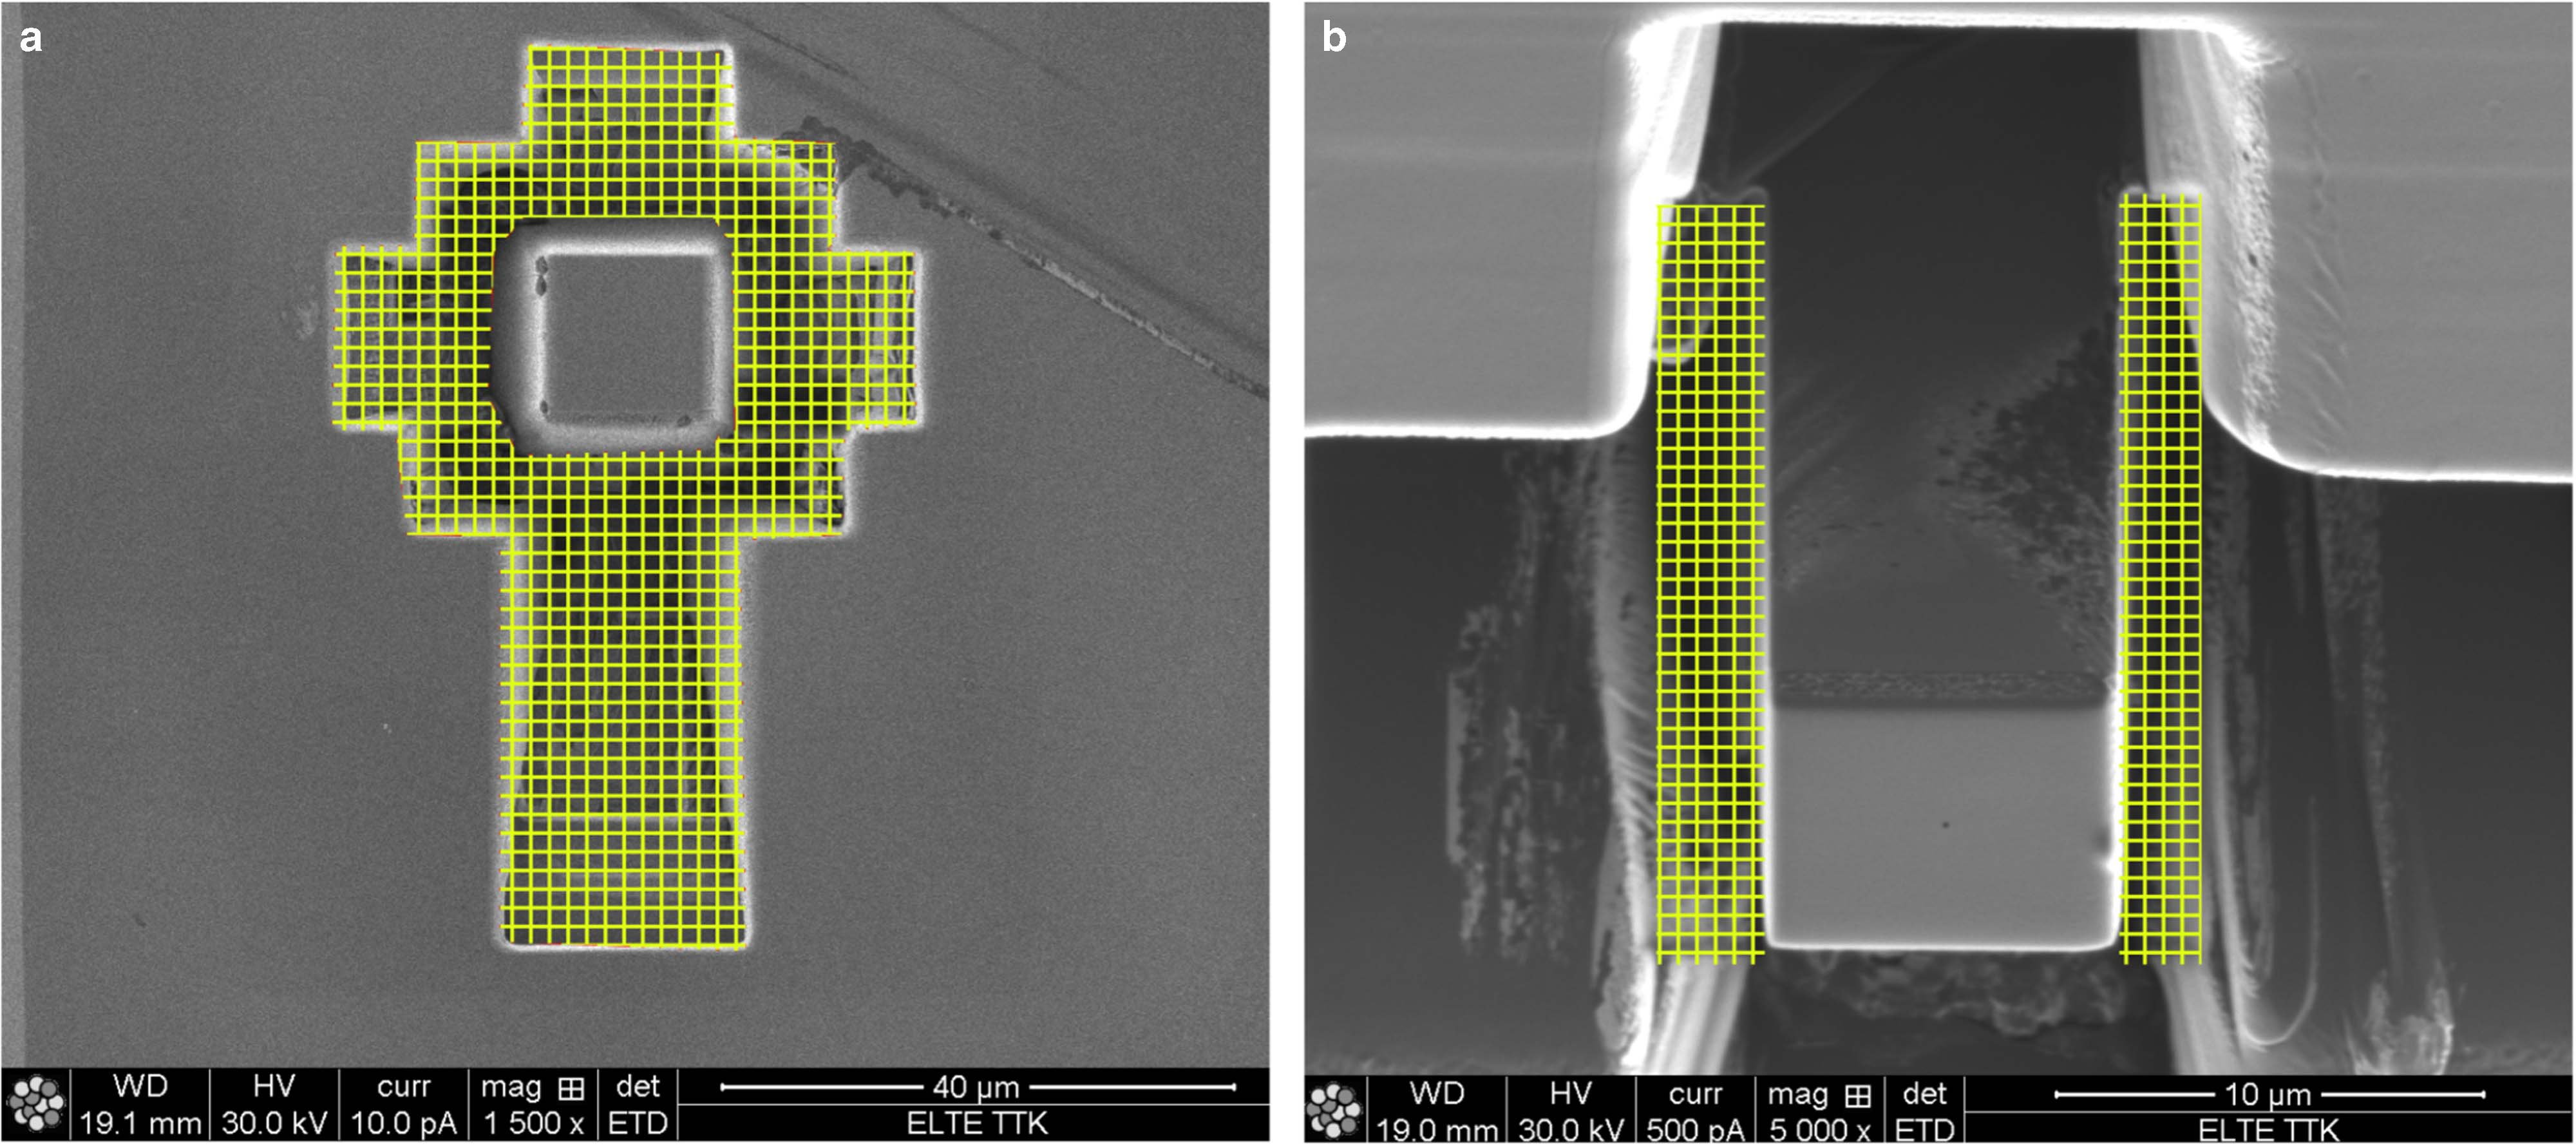
\includegraphics[width=1\textwidth]{Micron-Scale_Deformation2}
\caption[Raw and final pillar fabrication]{Both lathe and annular approaches were used during micropillar fabrication.\\
\textbf{(a)} The pillar was first hewed from the surface. FIB was directed from the point of view perpendicular to the surface marked by the yellow grid at \SI{30}{nA} current and at high voltage to create a whole around the pillar to fasten up further fabrication. The limb at the bottom provides a good view angle during the compression test. \\
\textbf{(b)} During the final milling step the sample was tilted by \SI{45}{\degree} and a smaller ion current of \SI{5}{nA} was used. The FIB was directed from the point of view to the yellow grid. In this step the top of the micropillar was already coated by a thin layer of Pt for protection.}
\label{fig:FIB_approaches}
\end{figure}

Apart from the rough digging mentioned in the first step, high milling angles were used in step~5. Despite the lower digging speed of the last milling steps the whole process were \numrange{2.5}{3} times faster then the commonly used perpendicular-only ion beam setup \cite{doi:10.1093/jmicro/dfh078}. The last step may also help to decrease the Ga ion implantation \cite{bei2007effects} even though it could be improved or revised \cite{greer2008comment}.

The following points sum up the most important features of the milling procedure proposed in this study.\begin{itemize}
\item Micropillars can be fabricated from any part of the flat surface of the bulk sample.
\item Micropillar preparation is touchless, thus damage or predeformation of the pillar can be arbitrary predefined or completely avoided during the the entire production procedure.
\item The final shape of the pillar is taper-free, i.e.\ the inclination of the side of the pillar was less than \SI{\pm0.5}{\degree}.
\item The method is considerably faster than the one suggested earlier, with a net mean milling time of less than \SI{4}{\hour} for the pillar size used in this study (\num{4 x 4 x 12}~\si{\micro m^3}).
\item FIB induced pillar hardening due to Ga implantation is decreased.
\end{itemize}

\begin{figure}[htbp!] 
\centering    
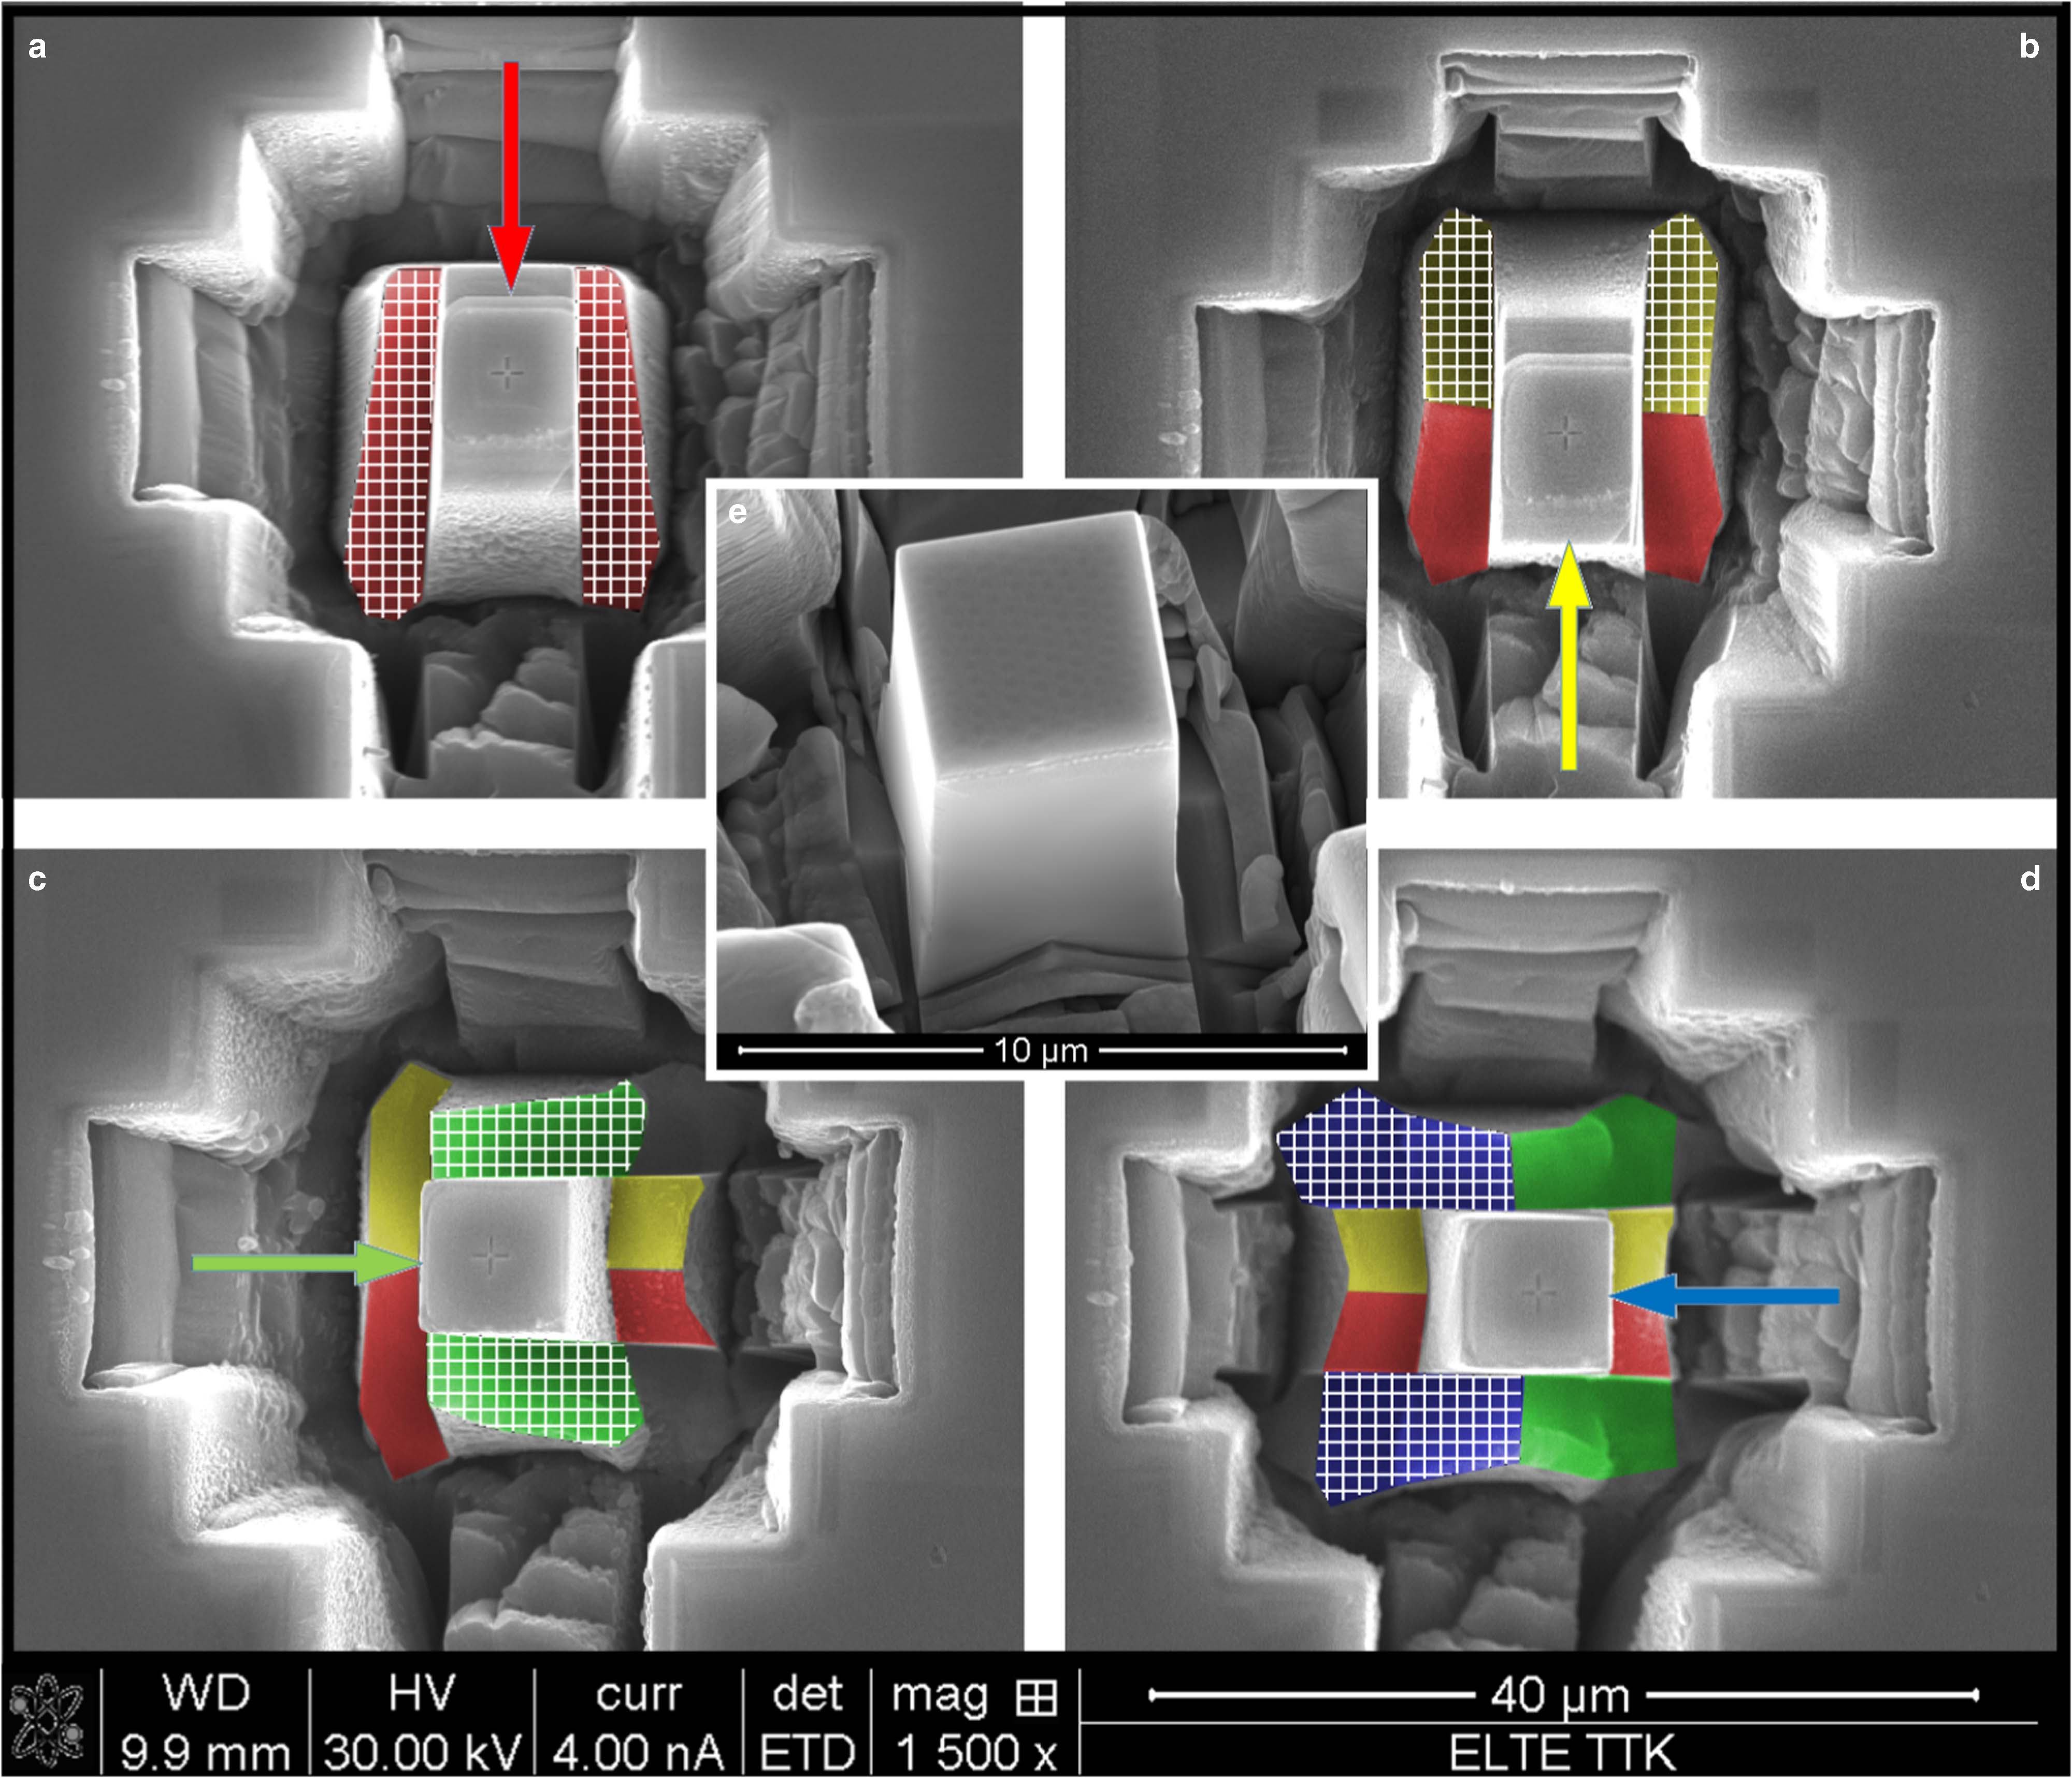
\includegraphics[width=1\textwidth]{Micron-Scale_Deformation}
\caption[Final pillar fabrication details]{Step~5 during pillar fabrication is detailed in this figure. Ion current was \SI{5}{nA}.\\
\textbf{(a)} Right after the raw pillar fabrication showed in Fig~\ref{fig:FIB_approaches}a. the sample was rotated around the pillar axis by a total of \SI{45}{\degree}. FIB was directed to two rectangular area merked by a red grid.\\
\textbf{(b)} The sample was rotated by \SI{180}{\degree} around the pillar axis. FIB was directed to the yellow grid to form the same sides of the sample but from the other direction.\\
\textbf{(c)} The sample was rotated by \SI{90}{\degree} around the pillar axis and the beam was directed to the green grid.\\
\textbf{(d)} The sample was rotated by \SI{180}{\degree} around the pillar axis to finish the shaping of the last two sides. FIB is directed onto the blue grid area.\\
\textbf{(e)} Steps \textbf{a-d} already gave a rectangular shaped pillar but to gain an even smoother shape they were repeated under \SI{1}{nA} first and \SI{0.1}{nA} second. The final pillar is shown in the inset.}
\label{fig:FIB_sides}
\end{figure}


\section{In situ device}
For an in situ micromechanical test the testing device has to fit into the vacuum chamber of the SEM. Although such compression devices are commercially available, an inexpensive yet faster device was developed in our laboratory. Our device easily fits into the vacuum chamber of a FEI Quanta 3D SEM\footnote{Produced by FEI, Hillsboro, Oregon, USA}. A schematic sketch is shown in Fig.~\ref{fig:nanotest}.

Two linear ultrasonic motors (denoted by X and Y in Fig.~\ref{fig:nanotest_schematic}) position the sample in the $x$ and $y$ directions. The AE detector is mounted on the top of the motors X and Y. In $z$ direction the sample can be moved by two motors. The first stage is moved by a gross linear step motor for raw movement moving the sample \SI{0.1}{mm} close to the indentation tip. The second stage is moved by a piezoelectric motor (piezoelectric positioning, PEP) with a resolution of \SI{0.1}{nm}. Only this stage is used for the compression test. The in-house fabricated spring -- which has a low longitudinal but high transversal stiffness -- is mounted onto the PEP stage and its movement is registered by the Z distance sensor, a capacitive sensor with a resolution of \SI{0.1}{nm}. With this latter two units both the deformation of the sample and the force can be determined. The deformation of the sample is $\epsilon = d-e$, where $d$ is the prescribed movement of the PEP stage (by Z fine) and $e$ is the measured elongation of the spring (by Z distance). The acting force can be calculated from $F=k \cdot e$, where $k$ is the spring constant determined from calibration. For pillar compression a flat punch diamond tip was used. To avoid static charges each item was grounded and a weakly conducting boron-doped tip was used.

To benefit from the high precision motors and sensors thermal and elastic elongation of the device must be prevented during the compression tests which take typically several minutes. To keep the temperature of the sample, X and Y motors constant, a Peltier cooling system was also mounted. The cold point of the cooling system was mounted onto the stage while the hot point was mounted onto the Quanta 3D SEM's appropriate, preconceived spot for Peltier cooling. This setup stabilised the temperature of the sample at \SI{15}{\celsius}. As the spring behave as an harmonic oscillator one has to deal with this disturbing effect. In an in-air environment air flows between the lamellae providing the necessary damping, but this is not the case in a vacuum chamber. Strong permanent magnets were installed next to the spring body to generate eddy current in order to provide the necessary damping.



\begin{figure}[htbp!] 
  \centering
  \begin{subfigure}[b]{0.48\textwidth}
    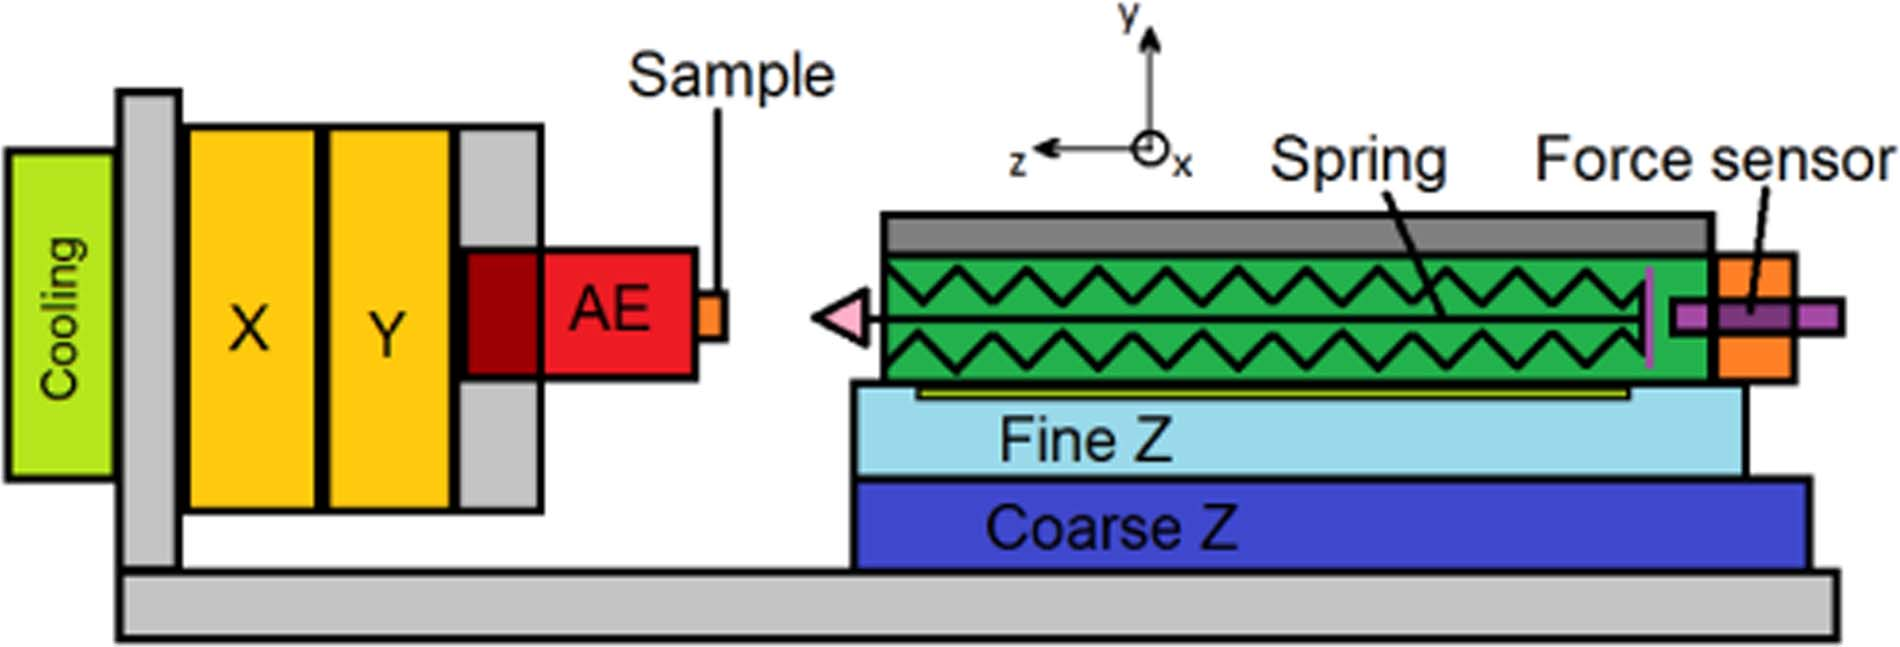
\includegraphics[width=\textwidth]{nanotest}
    \caption{The X, Y, Z fine, Z gross and Z distance sensor are commercially available products while the frame, the cooling, the spring and the suspension of the Z force motor are in-house designed.}
    \label{fig:nanotest_schematic}   
  \end{subfigure}
  \hspace{0.01\textwidth}      
  \begin{subfigure}[b]{0.48\textwidth}
    \includegraphics[width=\textwidth]{nanotest_spring}
    \caption{The spring and the well-suspended Z distance sensor together form the soft force-cell; the spring and the base of the suspension along with the tip holder is presented here in a mixed blueprint.}
    \label{fig:nanotest_spring}
  \end{subfigure}
  \caption[In situ device]{Schematic view of the in situ device developed in our laboratory for the NanoTest. The resonance of the device is marginal in-air but an issue inside the vacuum chamber, where magnetic damping can be used.}
  \label{fig:nanotest}
\end{figure}

To capture the phenomena caused by the PLC effect and dislocation avalanches, a minimum data collection rate of \SI{1}{k\hertz} is required along with a fast feedback controlling system, faster than any commercially available products. An analogous proportional-integral-derivative-type feedback electronics is developed in-house and used along with a fast 16 bit AD converter. The range and resolution parameters available for our device are summarised in table~\ref{table:nanotest_paramters}

\begin{table}[htbp]
\centering
\caption[NanoTest parameters]{The main parameters of our NanoTest device. The force sensor has two operating modes and can be improved or adjusted as the spring is interchangeable.}
\label{table:nanotest_paramters}
\begin{tabular}{llll}
\hline
\multicolumn{1}{c}{Part name} & \multicolumn{1}{c}{total range} & \multicolumn{1}{c}{resolution} & accuracy \\ \hline
X and Y stages  & \SI{\pm8}{mm}         & \SI{0.5}{\micro\meter} & \SI{0.01}{\micro\meter} \\
Z gross stage   & \SI{9}{mm}            & \SI{2}{\micro\meter}   & \SI{0.5}{\micro\meter}  \\
Z fine stage    & \SI{35}{\micro\meter} & \SI{1}{\nano\meter}    & \SI{0.1}{\nano\meter}   \\
Force sensor    & \SIlist{20;50}{mN}   & \SIlist{1;2.5}{\micro\newton} & \SIlist{1;2.5}{\micro\newton}   \\ \hline
\end{tabular}
\end{table}

\section{Acoustic emission measurements}
An AE measuring system was installed right below the sample to study the dynamic processes during the compression of the micropillars. An AE detector detects the transient elastic waves generated by fast elastic energy release processes. Such signals are originated from localised structural rearrangements, such as collective dislocation motion or twinning. As a consequence AE detectors can provide information on dynamic phenomena involved in plastic deformation \cite{heiple1987acoustic}.

AE signals can be used in bulk materials to identify the deformation mechanisms activated at different stages of the stress-strain curve \cite{BOHLEN2004214,PhysRevB.76.224110,dobrovn2009acoustic,KOVACS2014113}. The motion of single dislocation creates vibration with a characteristic energy below the sensitivity of AE detectors. At least dozens or hundreds of dislocations must move at the same time to generate an "audible" signal for AE detectors meaning that AE signals correspond to collective dislocation motion \cite{doi:10.1179/msc.1981.15.11-12.599}. AE detection was already used in bulk samples, as the crackling or avalanche-like plastic response does not only characterise micron-scale objects \cite{PhysRevB.76.224110}, but due to the huge number of simultaneously moving dislocations in bulk materials, the contribution of each avalanche to the total strain is smaller and smaller as the specimen size increases which results in a smooth stress-strain curve at a specimen size of a millimetre. Therefore AE can be a valuable technique on the macro scale to provide information about the underlying mechanism that cannot be revealed from the stress-strain curves solely. To our knowledge, the first successful investigation of AE signals from micron-sized pillars was performed in the framework of this study.

A Physical Acoustics PCI-2 acquistion board was used to capture and store the preamplified AE signals from the detector until the readout. A \SI{60}{\decibel} gain was applied on the direct signal of the detector between the frequency range from \SIrange{100}{1200}{kHz} then the board mentioned sampled the signal at a \SI{2}{MHz} rate between \SI{\pm 10}{V} using a \SI{18}{bit} A/D converter. The noise of the card (without detector) is \SI{17}{\decibel} and with the detector attached to the surface inside the vacuum chamber was not larger than \SI{24}{\decibel}, which is in agreement with the product bulletin provided by the product manufacturer. In our experiment a threshold level \SI{26}{\decibel} was used. The signal was recorded simultaneously with the stress and strain data.

The series of micropillars were fabricated from the same grain. The sample was pressed against the AE transducer using a metallic spring. To improve the acoustic contact, vacuum grease was also used to fill up the gap between the AE transducer and the sample.

A constant 	 strain rate were applied on the Al - 5\%Mg micropillar during the test. The calculated force and the AE signal recorded are plotted in Fig.~\ref{fig:loadAE_time}. As it can be seen in the figure the sample shows the well-known PLC instability. It is suspected that the stress drops correspond to the collective depinning of the dislocations from the solute atoms as obstacles generating a measurable AE signal marked by the four red lines. From  the negative slope of stress-real strain curve one can identify the strep-drops.

\begin{figure}[htbp!] 
\centering    
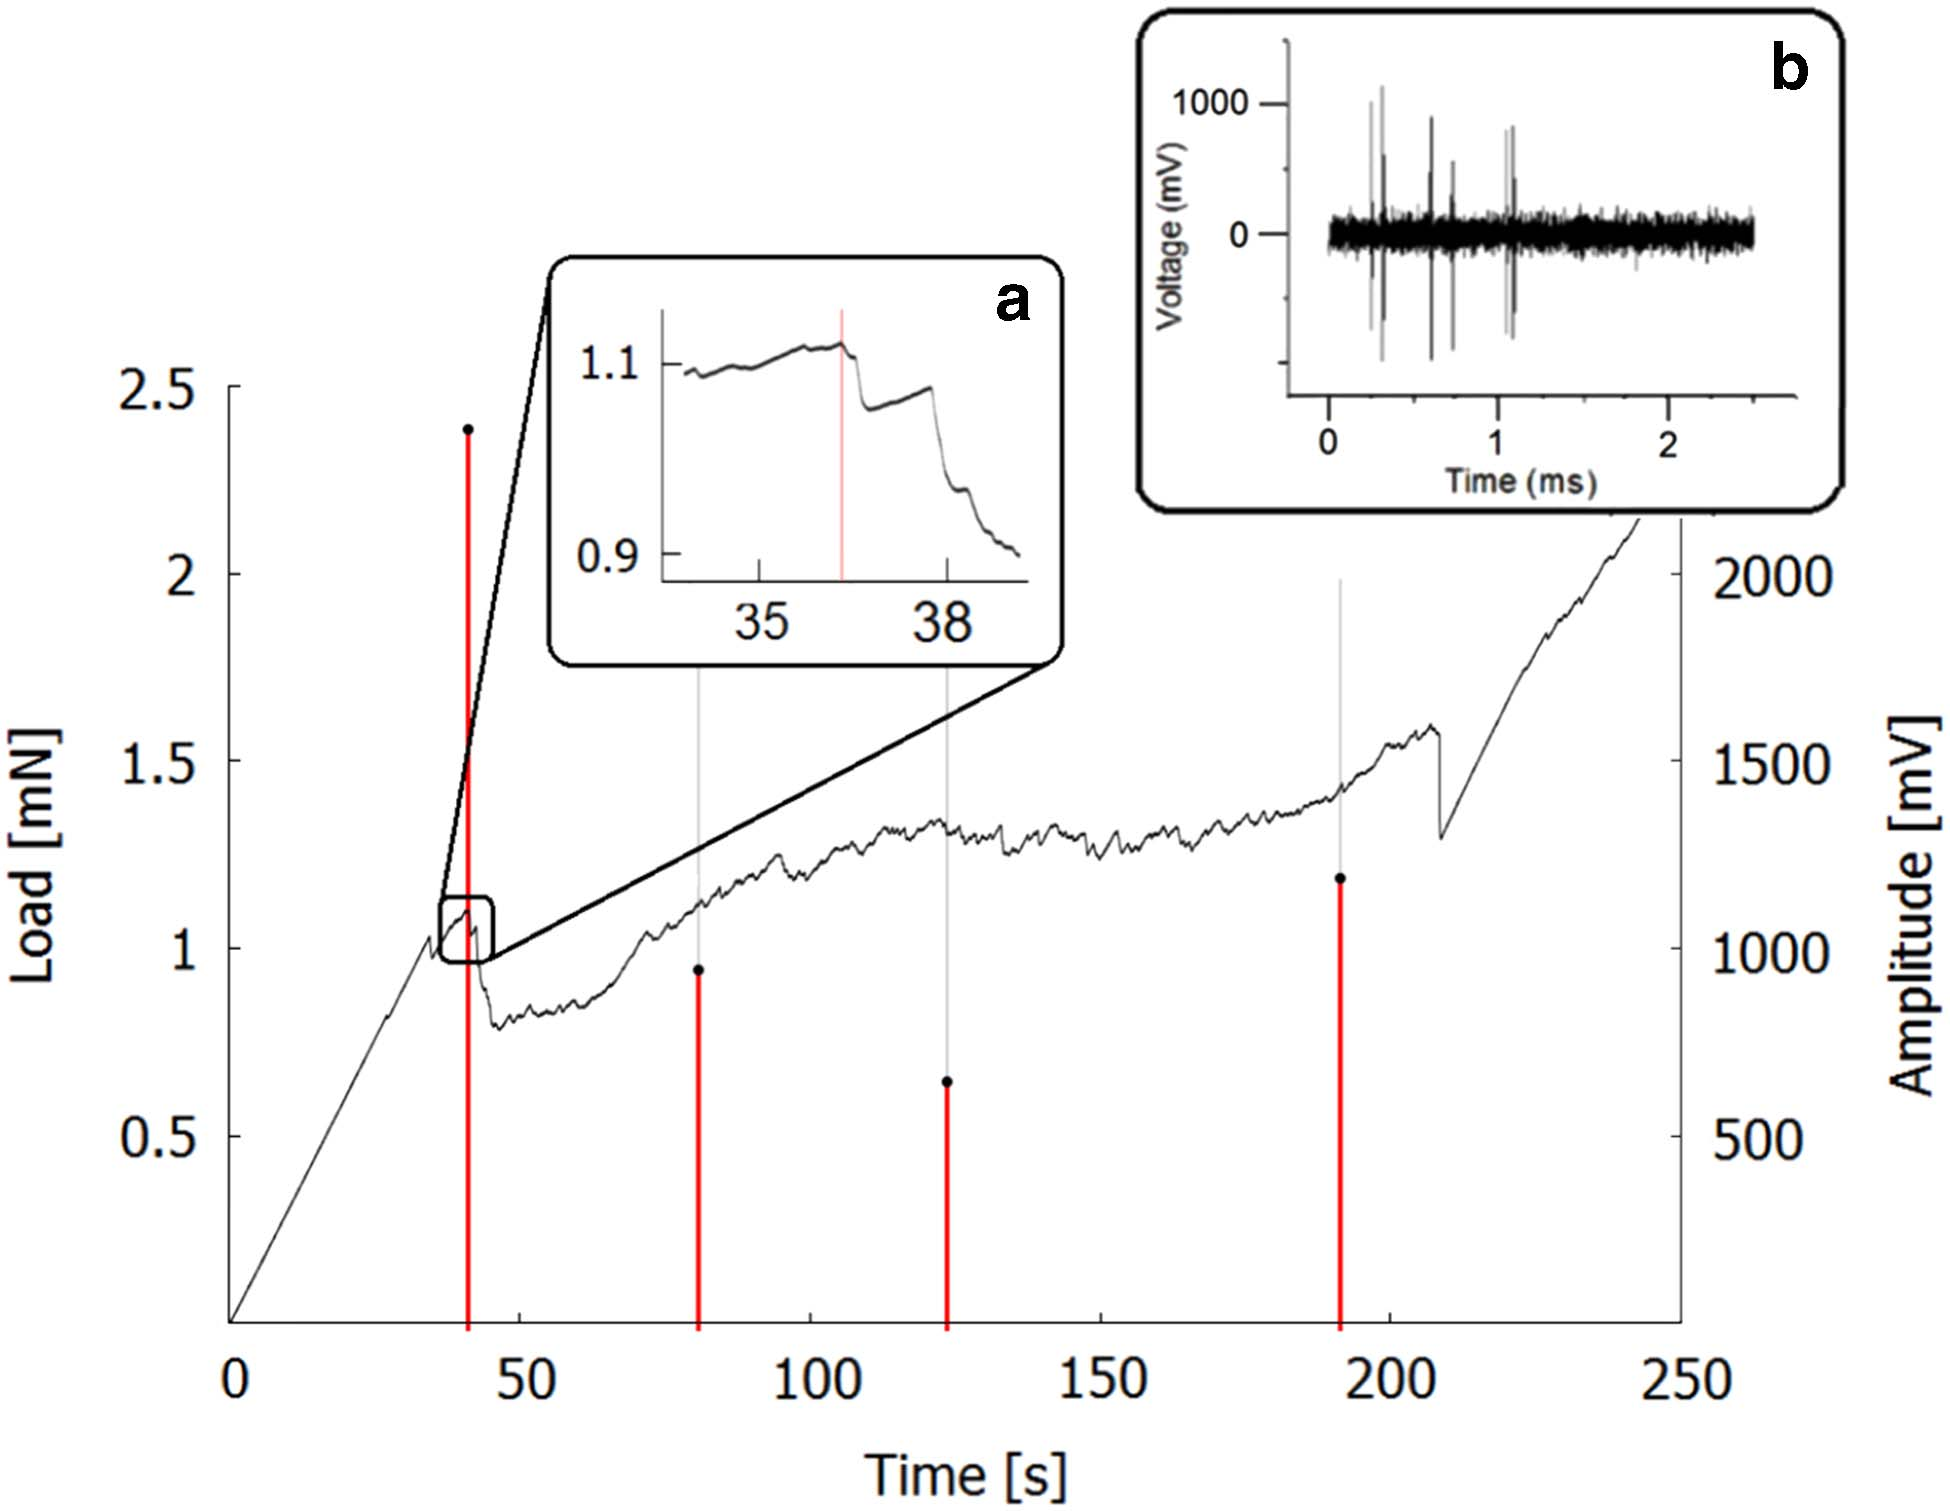
\includegraphics[width=0.6\textwidth]{Micron-Scale_Deformation3}
\caption[Load curve and AE signals]{The load and the local maximum of the AE signal versus time obtained from a micropillar compression test under constant strain rate are plotted.\\
\textbf{(a)} Inset \textit{a} shows a typical stress drop enlarged.\\
\textbf{(b)} Inset \textit{b} shows the waveform of an individual AE peak on a \si{m\second} scale.}
\label{fig:loadAE_time}
\end{figure}

Further investigations are required to unfold how stress drops caused by the PLC instability differ from the stress drops caused by dislocation avalanches. Such a comparison could be set up using non-PLC capable pure Al micropillars. As seen in Fig.~\ref{fig:loadAE_time}a, large AE signal is detected right before the onset of the stress drop. The PLC effect can suppress or at least compete with the intrinsic intermittent dislocation motion originated from dislocation avalanches, especially at size scale of the fabricated micropillar (\SI{4x4x12}{\micro m^3}). This two effects screen the well-known periodic stress drop structure of the stress-strain curve by introducing uncorrelated stress-drops due to dislocation avalanches.

The distinguishable large peaks in the acoustic signal shown in Fig.~\ref{fig:loadAE_time}b indicate that AS signal detection related to dislocation avalanches may be feasible even for samples with a small volume of \SI{100}{\micro m^3}.

\section{Summary}
The plastic response caused by the external stress shows intermittent characteristic at the micron scale, a phenomenon not observed in bulk samples. Although the stress-strain curve from compression test differs in general from sample to sample but they may share similar behaviour and an approach based on statistical investigation can be suitable to unravel the underlying stochastic processes and identify some parameter characterising the system examined. Therefore numerous tests must be performed requiring micropillars are needed. For that reason the efficiency of the technique used for micropillar fabrication must be improved in order to produce micropillars in a number suitable for statistical ensembling.

A high precision, fast-feedback micromechanical compression device was developed in our laboratory to measure the stress and strain during the compression with extra care. All the data and the in situ SEM arrangement validate the plausible assumptions based on AE signal detection. The unit of the three mutually supportive investigation method gives an original tool suitable to perform micromechanical tests at the aim of revealing the stochastic properties of micron scale plasticity.

\section*{Notes in regard to the thesis}
In this study technological advancement in micropillar fabrication and compression were introduced. It is well emphasised how important they are in order to start mass investigation on micron scale plasticity and a demonstrative example was also given. At this stage one cannot compare yet the properties of micron scale plasticity obtained theoretically with the ones observed experimentally in this study, but the step made here is elementary necessary to achieve this goal. Ongoing research with new results are already available but not achieved the state of a publishable level.

My specific contribution to this study is the following. I played a role in the selection and pretreatment of the cast aluminum and I was also involved in the dislocation density measurement performed by X-ray line profile analysis. I played a major role in the whole process of the development of the force sensor from design until calibration. Even though many times it required abilities not associated with the skills of a doctoral student in physics, these engineering-like challenges must have been solved to take a step further in the field of micron scale plasticity.

I look forward for challenges in the improvement of the force sensor, the AE signal detection and the data analysis. I believe the resource requested is given to fabricate numerous PLC and non-PLC micropillars, the compression test would serve valuable information on their behaviour and a comparison with bulk samples could provide the next step further for characterising micron scale plasticity.

